\documentclass[preview]{standalone}
\usepackage{tikz}
\usepackage{pgfplots}
\pgfplotsset{compat=1.14}
\usetikzlibrary{arrows,decorations.markings}
\usetikzlibrary{matrix,calc,shapes}
\usepgfplotslibrary{fillbetween}
\tikzset{
	treenode/.style = {shape=rectangle, rounded corners,
		draw, anchor=center,
		text width=5em, align=center,
		top color=white, bottom color=blue!20,
		inner sep=1ex},
	decision/.style = {treenode, diamond, inner sep=0pt},
	root/.style     = {treenode, font=\Large, bottom color=red!30},
	env/.style      = {treenode, font=\ttfamily\normalsize},
	finish/.style   = {root, bottom color=green!40},
	dummy/.style    = {circle,draw}
}

\begin{document}
%  \documentclass[tightpage]{standalone}


% \usepackage[active,pdftex,tightpage]{preview}
% \PreviewEnvironment[{[]}]{tikzpicture}
%  \usepackage{tikz}
%  \usepackage{pgfplots}
%  \pgfplotsset{compat=1.15}
% \begin{document}

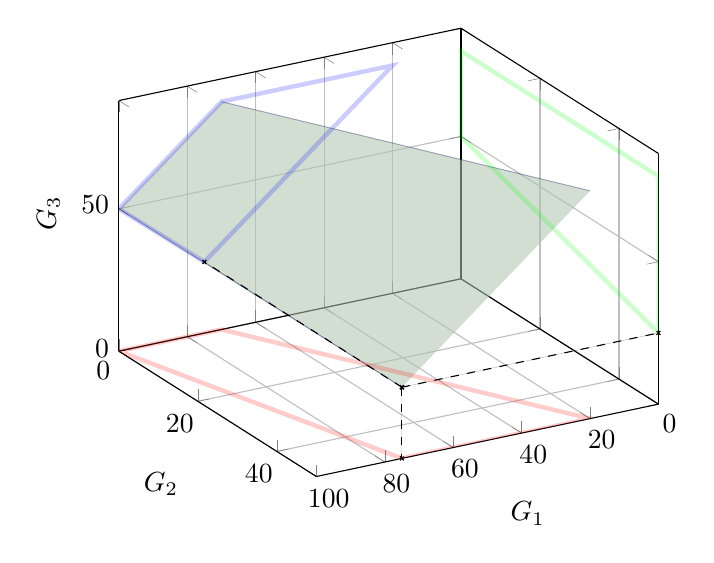
\begin{tikzpicture}
\begin{axis}[
%	width=0.95\textwidth,
%    height=0.75\textwidth,
grid=both,view={-210}{30},
% colorbar horizontal,
colormap/viridis,
% colormap={whitered}{color(0pt)=(white) color(1pt)=(red) color(2pt)=(white) color(3pt)=(red) color(4pt)=(white) },
% opacity=1,
% xmin=0,
% xmax=90,
% ymin=0,
% ymax=50,
zmin=0,
% zmax=80,
xlabel={$G_1$},
ylabel={$G_2$},
zlabel={$G_3$},
]


\addplot3[name path=path1,fill=blue, opacity=0.1, fill opacity=0.4,samples=2] coordinates{
	(75,50,25) 
	(100,0,50)};

\addplot3[name path=path2,fill=blue, opacity=0.1, fill opacity=0.4,samples=2]  coordinates{
	(20,50,80)
	(70,0,80)
};

\addplot [green, opacity=0.1] fill between[of=path1 and path2];

\draw[ultra thick,draw=red,fill=none,opacity=0.2]
(70,0,0)--(100,0,0)--(75,50,0)--(20,50,0)--cycle;


\draw[ultra thick,draw=blue,fill=none,opacity=0.2]
(75,0,25)--(100,0,50)--(70,0,80)--(20,0,80)--cycle;

\draw[ultra thick,draw=green,fill=none,opacity=0.2]
(0,0,50)--(0,0,80)--(0,50,80)--(0,50,25)--cycle;


\addplot3[dashed,mark=x,mark size=1,mark options=solid,fill=black] coordinates
{(75, 50, 25)
	(75, 50, 0) };

\addplot3[dashed,mark=x,mark size=1,mark options=solid,fill=black] coordinates
{(75, 50, 25)
	(75, 0, 25) };


\addplot3[dashed,mark=x,mark size=1,mark options=solid,fill=black] coordinates
{(75, 50, 25)
	(0, 50, 25) };

%(70,0)--(100,0)--(75,50)--(20,50)--cycle;


\addplot3[name path=path1,fill=blue, opacity=0.1, fill opacity=0.4,samples=2] coordinates{
	(75,50,25) 
	(100,0,50)};

\addplot3[name path=path2,fill=blue, opacity=0.1, fill opacity=0.4,samples=2]  coordinates{
	(20,50,80)
	(70,0,80)
};

\addplot [lightgray, opacity=0.5] fill between[of=path1 and path2];

\end{axis}
\end{tikzpicture}


% \end{document}\\





\end{document}
